\section{Various technicalities \label{sec:subtleties}}

In this section, we discuss some subtle points of our construction. 


\subsection{Stability of the reconstructed bulk operators/``spread of the transfer function''}

A possible objection to our construction is the following: in Schwarzschild coordinates, an infalling observer never crosses the horizon, since the point of crossing formally has Schwarzschild time $t\rightarrow \infty$. Moreover, the  ``time'' of the gauge theory is naturally identified with the Schwarzschild time in the bulk. These statements together may be taken as an indication that in order to reconstruct local operators at and behind the horizon, we need information from the gauge theory {\it for all times}. If true, this could be a serious problem since we expect the late time behavior of pure states to have significant variance due to Poincare recurrences and other kinds of statistical fluctuations, including ${1 \over N}$ 
corrections that might pile up over time.

The same conclusion seems to follow if one (wrongly) assumes that the support of the operator $\phi_{\rm CFT}(t,\vect{x},z)$ is mostly localized on the intersection of the boundary of AdS with the spacelike cone emanating from the point $(t,\vect{x},z)$. This (wrong) assumption seems to suggest that as the point moves close to the horizon, the support of the operator spreads over the entire boundary and moreover it becomes difficult to understand what happens when the point moves behind the horizon.

Fortunately these arguments are not really correct and we will explain that the reconstructed bulk observables $\phi_{\rm CFT}(t,\vect{x},z)$ only require knowledge of the boundary fields for (approximately) a finite interval in boundary time, which can be made parametrically smaller, in the large $N$ limit, from time scales related to fluctuations and recurrences. 



We believe that our momentum space formulation helps us get a sharp sense of the accuracy of our construction. In particular, the question above can be converted to the following questions:
\begin{enumerate}
\item
From a measurement of boundary correlators, with a given accuracy and over a certain time-scale, how accurately can we extract the modes ${\cal O}_{\omega,\vect{k}}$ that we require above.
\item
Can a small inaccuracy in the ${\cal O}_{\omega,\vect{k}}$ modes get blown up to a large inaccuracy in the reconstructed bulk fields $\phi_{\rm CFT}$.
\end{enumerate}

Let us start with the first question.  Let us say that we  measure the correlator on the boundary for a {\em finite time interval} $[0,T]$. (It is trivial to do a similar analysis for the spatial coordinates, but for simplicity, we focus on time here.) Moreover, the observer samples this correlator at short-time intervals $t_{uv}, 2 t_{u v}, \ldots$ for a total number of samples ${T \over t_{uv}}$. (We will take this to be an integer to lighten the notation.) Using this procedure how accurately  can we discern the various frequencies? 

Let us say that the original correlator is $C(t) = \int C_{\omega} e^{-i \omega t}$. By doing a discrete Fourier transform using the sample points above, we can measure the frequency modes
\be
\label{measuredc}
\hat{C}\left({2 \pi \nu \over T} \right) =  {t_{u v} \over T} \sum_{j = 0}^{{T \over t_{u v}} - 1} \int C_{\omega} e^{-i \omega j \over T} e^{2 \pi i \nu j \over T} d \omega = \int C_{\omega} R_{\omega} d \omega 
\ee
with 
\be
R_{\omega} = {t_{uv} \over T} \frac{e^{i T (2 \pi  \nu -\omega )} -1}{e^{ i t_{uv} (2 \pi \nu - \omega)}-1 }.
\ee
We remind the reader (see figure \ref{spreadfuncplot}) that if $\omega t << 1$ and $\omega T >> 1$, then $R_{\omega}$ is a sharply peaked function with a maximum of $1$ at $\omega = 2 \pi \nu$.
\begin{figure}
\begin{center}
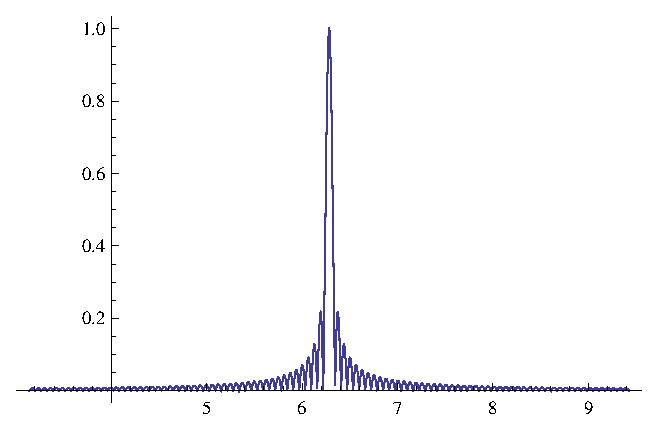
\includegraphics[height=5cm]{spreadfunc.eps}
\caption{$R_{\omega}$ with $\nu = 1$ \label{spreadfuncplot}}
\end{center}
\end{figure}
 
On the other hand, if $\omega$ is a very low frequency --- signals at ultra-low frequencies can be produced by phenomena like Poincare recurrence --- then \eqref{measuredc} is negligible except at $\nu = 0$. So these frequencies do not contaminate the measurement of Fourier modes with higher frequencies.

Similarly, \eqref{measuredc} also tells us that if we wish to measure
the Fourier mode to some accuracy ${1 \over N^{\alpha}}$, then we can do
that by measuring the real-time signal to the same accuracy --- we do not
require any parametric enhancement of accuracy at low frequencies.

So we reach the expected conclusion it is possible measure the Fourier modes
of the operator ${\cal O}_{\omega, \vect{k}}$ between some IR-cutoff ${1 \over T}$ and some UV-cutoff ${1 \over t_{uv}}$ to any given accuracy
by sampling position correlators at intervals smaller than $t_{uv}$ and for a length of time larger than $T$, with the same accuracy.














Having now established that the Fourier modes ${\cal O}_{\omega, \vect{k}}$ 
can be measured in principle, the next question has to do with whether
low frequency modes become very important near the horizon. In order to do that we consider the bulk 2-point function of our local operators $\phi_{\rm CFT}(t,\vect{x},z)$.

\subsubsection{Outside the horizon}
First we start with points outside the horizon. We have
\begin{align*}
&{1 \over Z_{\beta}} {\rm Tr}\Big(e^{-\beta H} \phi_{\rm CFT}(t_1,\vect{x}_1,z_1)  \phi_{\rm CFT}(t_2,\vect{x}_2,z_2)\Big)  \\
&= (2\pi)^d \int_{\omega>0} {d\omega \over (2 \pi) 2 \omega} {d^{d-1}\vect{k} \over (2 \pi)^{d-1}}\, \begin{aligned}[t] \Bigg[&\hat{f}_{\omega,\vect{k}}(t_1,\vect{x}_1,z_1) \hat{f}^*_{\omega,\vect{k}}(t_2,\vect{x}_2,z_2) {e^{\beta \omega}
\over e^{\beta \omega}-1} \\ & + 
 \hat{f}^*_{\omega,\vect{k}}(t_1,\vect{x}_1,z_1) \hat{f}_{\omega,\vect{k}}(t_2,\vect{x}_2,z_2) {1
\over e^{\beta \omega}-1} \Bigg]
\end{aligned}
\end{align*}
Here we used the definition of the bulk operators \eqref{upliftb} and the thermal expectation values of the Fourier modes $\hat{\cal O}_{\omega,\vect{k}}$ that we discussed around equation \eqref{thermaloca}. Remember that the hatted modes $\hat{f}_{\omega,\vect{k}}(t,\vect{x},z)$ are those which are canonically normalized with respect to the Klein Gordon norm.

The question about the late-time sensitivity is a question about the region of this integral around $\omega=0$. First we notice that we have an explicit factor of ${1\over \omega}$. Second, the thermal factors ${e^{\beta\omega}\over e^{\beta\omega}-1}$ and ${1\over e^{\beta\omega}-1}$ both go like ${1\over \beta \omega}$ for low $\omega$. Third, the modes have the property that for fixed $(t,\vect{x},z)$ we have that $\hat{f}_{\omega,\vect{k}}(t,\vect{x},z)$ goes to zero linearly with $\omega$ for small $\omega$. This can be verified explicitly in the case of the modes on a BTZ background (see appendix \ref{appendix2dthermal}) but is also true for other black holes. All in all we find that if we keep the points fixed and consider low $\omega$, the integrand goes like $\omega^0$ and hence the integral converges.

Since the integral is convergent in the limit $\omega=0$, it means that the sensitivity of the operator $\phi_{\rm CFT}(t,\vect{x},z)$ to the region of small $\omega$ (or equivalently ``late-time'' in position space) is actually small. In order to demonstrate this let us consider the order of various limits a bit more carefully. Let us consider the reconstructed local bulk operator \eqref{uplifta}, but with the inclusion of an IR cutoff $\delta$ in frequency space
\[
\phi_{\rm CFT}^{\delta}(t,\vect{x},z) \equiv \int_{\omega>\delta}{d\omega d^{d-1}\vect{k} \over (2\pi)^d}\, \left[{\cal O}_{\omega,\vect{k}} \, f_{\omega,\vect{k}}(t,\vect{x},z) + {\cal O}_{\omega,\vect{k}}^\dagger \, f_{\omega,\vect{k}}^*(t,\vect{x},z)\right]
\]
The operator $\phi_{\rm CFT}^{\delta}$ is not exactly the same as our original operator $\phi_{\rm CFT}(t,\vect{x},z) =\phi^{\delta=0}_{\rm CFT}$ defined in \eqref{uplifta}. However, since the integral is convergent in the region of $\omega=0$, the difference between correlation functions of $\phi^\delta_{\rm CFT}$ and correlation functions of $\phi^{\delta=0}_{\rm CFT}$ goes to zero as $\delta\rightarrow 0$.

Coming back to the question about the sensitivity to the details of the pure state: suppose we want to reconstruct the bulk with some  ``resolution'' $\epsilon$ (which we take to be $N$-independent). For any given $\epsilon$ there is an IR cutoff $\delta$, such that the correlators of $\phi_{\rm CFT}^\delta(t,\vect{x},z)$ reproduce those of a local bulk field up to the accuracy $\epsilon$, {\it if the boundary correlators agreed with the thermal ones, down to the IR frequency cutoff $\delta$}. But for any given and fixed IR cutoff $\delta$ in frequency space, we can take $N$ to be large enough, so that the boundary correlators on a typical pure state agree with those of the thermal ensemble down to $\omega \approx \delta$.

Putting everything together, we find that for any desired ``resolution $\epsilon$'', it is possible to take $N$ to be large enough and to ensure that the details of the typical pure state become unimportant.


\subsubsection{Inside the horizon}

In order to reach the same conclusion for points behind the horizon, we need to demonstrate that the integral over $\omega$ in the 2-point function for points behind the horizon, is well-behaved around $\omega=0$. Here the situation is more interesting. The reconstructed bulk operator is given by \eqref{finalbehind}, that is
\[
 \phi^{\rm II}_{\text{CFT}}(t,\vect{x},z) =
\int_{\omega>0} {d\omega d^{d-1}\vect{k} \over (2 \pi)^d} \left[ {\cal O}_{\omega,\vect{k}}\, g_{\omega,\vect{k}}^{(1)}(t,\vect{x},z) + \widetilde{\cal O}_{\omega,\vect{k}} \,g_{\omega,\vect{k}}^{(2)}(t,\vect{x},z)+ {\rm h.c.}
\right]
\]
When computing the 2-point function of this operator we find several contributions coming from the 2-point functions of the  ``usual'' modes ${\cal O}_{\omega,\vect{k}}$, from the 2-point functions of the  ``tilde'' modes $\widetilde{\cal O}_{\omega,\vect{k}}$, as well as from cross-terms between the two.

If we focus on the contribution to the 2-point function coming from the terms $\langle {\cal O}_{\omega,\vect{k}}
{\cal O}^\dagger_{\omega',\vect{k}'}\rangle_\beta$ and $\langle {\cal O}_{\omega,\vect{k}}^\dagger {\cal O}_{\omega',\vect{k}'}\rangle_\beta$ we find that the integral over $\omega$ is divergent from the $\omega=0$ region. This is the Fourier-space manifestation of the arguments mentioned in the first two paragraphs of this section. It might seem that this small $\omega$ divergence would invalidate our claims.

However, instead of focusing only on {\it some} of the terms contributing to the 2-point function, if we consider the contribution from all terms together, i.e. including the ``tilde'' modes (and the cross terms) we find that the integral over small $\omega$ becomes convergent! The divergence encountered above when considering the modes ${\cal O}_{\omega,\vect{k}}$ alone, disappears when we consider both ${\cal O}_{\omega,\vect{k}}$ and $\widetilde{\cal O}_{\omega,\vect{k}}$ together!

This means that there is a specific way to reorganize the terms in the integral over $\omega$, so that the integral becomes manifestly convergent for small $\omega$. It turns out that if we group together the modes ${\cal O}_{\omega,\vect{k}}$ with the $\widetilde{\cal O}_{\omega,\vect{k}}$ in the natural ``Kruskal'' combinations
\[
 {\cal K}^{(1)}_{\omega, \vect{k}} = {{\cal O}_{\omega,\vect{k}} - e^{-{\beta \omega\over 2}} \widetilde{\cal O}_{\omega,\vect{k}} \over \sqrt{1-e^{-\beta \omega}}}\qquad,\qquad
{\cal K}^{(2)}_{\omega, \vect{k}} =  {\widetilde{\cal O}_{\omega,\vect{k}}^\dagger - e^{-{\beta \omega\over 2}}{\cal O}^{\dagger}_{\omega,\vect{k}} \over \sqrt{1-e^{-\beta \omega}}}
\]
then the integral is manifestly convergent for small $\omega$. The Kruskal creation operators are, of course, just given by the Hermitian conjugates
of the relations above.

As a matter of fact, this situation can also be studied in the case of Rindler space, where the modes are easy to write down explicitly. We present the analysis in appendix \ref{rindlerq}. In Rindler space, when computing the 2-point function for points behind the ``Rindler horizon'', we find the same small $\omega$ divergence, when considering the contribution from only one set of modes. 
We can check explicitly that the divergence disappears if the modes are grouped together in the ``Unruh modes''. The relation between the Unruh and the Rindler modes given in \eqref{unruh} is precisely the same as the relation between the Kruskal and the AdS-Schwarzschild modes above.


To summarize, for points behind the horizon the integral over small $\omega$ is still convergent, which means that the sensitivity of the bulk 2-point function to the low $\omega$ (or late time) boundary correlators is small. The argument about the order of limits mentioned in the previous subsection can be repeated
in identical form, and we conclude that the reconstructed black hole region II is --- in the large $N$ limit --- insensitive to the details of the specific pure state.


\subsubsection{What happens exactly on the horizon?}
At the horizon, the mode functions do not diverge but they start oscillating very rapidly. We can see this from the formula \eqref{psinearh}. Near the horizon, in terms of the coordinates $U$ and $V$ defined in section \ref{secadseternal}, the modes are simply
\[
\hat{f}_{\omega, \vect{k}} = e^{i \vect{k} \cdot \vect{x}} \left(e^{i \delta_{\omega, \vect{k}}} e^{-2 \pi \zhor \omega \over d} U^{2 i \zhor \omega \over d} + e^{-i \delta_{\omega, \vect{k}}} V^{-2 i z_0 \omega \over d} \right)
\]
Let us say that we have been able to measure boundary modes accurately up to some frequency ${2 d \over \zhor N^{\alpha}}$. ($\zhor$ is a natural scale since it also sets the temperature.)  Near the future horizon, which is at $U = 0$, modes below
this frequency become important only for 
\be
\label{breakdownregion}
\ln(U) \sim -N^{\alpha} \Rightarrow U \sim e^{-N^{\alpha}}.
\ee
It is only in this region that our construction starts to develop inaccuracies.

In fact the proper time taken by the infalling observer to cross the region \eqref{breakdownregion} is itself exponentially suppressed in $N$. It is unclear to us whether it is possible even, in principle, to speak of the experience of the infalling observer over such a short time scale. If we {\em average} over the experience of the observer as he crosses the black hole, over some time scale that is larger than this --- even a time scale that is power law suppressed in $N$ and scales like $\Or[{1 \over N^{\alpha}}]$ --- then we see that the tiny frequencies that we have neglected on the boundary do not cause any difficulties. 




\subsection{Pure vs thermal states}

A tacit assumption in our analysis in sections \ref{sec:behind} and \ref{sec:outside} was that correlators of the operator $\phi_{\rm CFT}(t,\vect{x},z)$ in a ``typical'' heavy pure state are the same as its correlators in
the thermal ensemble. This is consistent with general intuition from statistical mechanics and it was on this basis that we concluded that an infalling observer will not notice anything special as he falls through the horizon, when the black hole is in a pure state.


The argument from the beginning of section \ref{subsechorizonnat} provides further weight to this expectation. In that section, we argued that if
correlators of light operators factorize on a typical heavy pure state
then these correlators cannot be used to distinguish between various typical pure states $|\Psi \rangle$ in the thermal ensemble. More precisely, our arguments suggest that by measuring these correlators to an accuracy ${1 \over N^{\alpha}}$, we could divide these pure states into $\Or[N^{\alpha}]$ different classes but still not pinpoint which one we are in since there are $\Or[e^{-N}]$ different states in the ensemble. 

But, how do we know that factorization holds in a pure state? Even if 
factorization holds for thermal correlators --- and we might be able
to make an argument for this by applying the usual power counting
arguments to the Feynman diagram expansion of these correlators in the 
Schwinger-Keldysh formalism --- it is not obvious that this carries over to pure states.

However, the argument for this is simple. The key point is that the question of how different an observable $A$ is, on a typical pure state, from the same observable on the thermal ensemble, is a question about the {\it variance} of the observable across the ensemble of all pure states. This can be estimated from computing the {\it thermal expectation value of the square of the observable}. 

In other words the variance of $A$ across different pure states can be related to the following quantity {\it which can be computed within the thermal ensemble}
\be
\label{variance}
{1 \over Z_{\beta}} {\rm Tr}(e^{-\beta H} A^2) - {1 \over Z_{\beta}^2} {\rm Tr}(e^{-\beta H}A)^2  
\ee

Let us apply this measure to the observable 
\[
A = {\cal O}_{\omega_1, \vect{k_1}}  {\cal O}_{\omega_2, \vect{k_2}}  {\cal O}_{\omega_3, \vect{k_3}}  {\cal O}_{\omega_4, \vect{k_4}}   -  {1 \over Z_{\beta}^2} {\rm Tr} \left(e^{-\beta H} {\cal O}_{\omega_1, \vect{k_1}}  {\cal O}_{\omega_2, \vect{k_2}} \right)  {\rm Tr} \left(e^{-\beta H} {\cal O}_{\omega_3, \vect{k_3}}  {\cal O}_{\omega_4, \vect{k_4}} \right)- \ldots,
\]
where $\ldots$ indicate the other
products of two point functions that enter here. Then the fact that 
the expectation value of $A$ and its powers vanishes in the thermal ensemble up to ${1 \over N}$ means that no ``appreciable'' class of pure states can have non-vanishing $A$.

One might also wonder about the significance of $\Or[1]$ variance of
the operators given in \eqref{thermaloca} and \eqref{thermalocab}. In fact
this variance has a natural semi-classical interpretation: it just indicates the statistical fluctuations in the thermal gas of particles that 
surround the black hole. These fluctuations do not modify the leading order geometry, since they are an $O(1)$ and not $O(N^2)$ effect and thus cannot backreact in the large $N$ limit. Moreover the amount of information 
contained in them, as we argued before, is parametrically smaller than that of the entropy of the black hole itself.







\subsection{Definition of tilde operators}
As the reader will have noticed, the construction of the $\widetilde{\cal O}$ operators in section \ref{sec:behind} suggests that the precise Heisenberg operators $\widetilde{\cal O}$ that an observer will encounter may differ quite significantly depending on which pure state the black hole is in. The important point is that this non-uniqueness is unimportant from an operational point of view. The bulk observer lives in a particular black hole microstate. By measuring correlators that involve a finite number of bulk fields $\phi$, the observer can only infer that the $\widetilde{\cal O}$ operators {\em effectively} satisfy the same algebra as the ${\cal O}$ operators. The reader may wish to consult the toy model in section \ref{sec:toy} for an explicit construction of the $\widetilde{\cal O}$ operators, where this dependence on the state and its operational insignificance can both be seen. 

The $\widetilde{\cal O}$ operators also depend on the specific division of the CFT Hilbert space into a coarse and a fine grained part. Once again, this dependence is not operationally significant. This property can also be seen in the toy model of section \ref{sec:toy}. 
\subsection{Do our operators describe the ``real'' infalling observer?}
A question that we have commonly encountered is: ``how do we know that this description corresponds to the `real' experience of the infalling observer.'' 

Before we address this, let us briefly emphasize a philosophical point, which is uncontroversial and even seemingly banal.  Let us say that we are given a quantum system ${\cal Q}$ and that in some approximation the accessible observables in this system can be re-organized into observables $\phi^{(i)}(\vect{x})$, where ${\vect{x}}$ are points on some manifold ${\cal M}$ and, and $i$ is some index that labels the operator in question.  Moreover if the correlators of these operators are the same as the correlators of perturbative fields propagating on ${\cal M}$, then the system ${\cal Q}$ is indistinguishable from the system describing perturbative fields on ${\cal M}$. 

In this paper, we have shown that the natural observables of a CFT with large $N$ factorization can be reorganized, at leading order, into the correlators of a non-local CFT operator $\phi_{\text{CFT}}(t, \vect{x}, z)$, which is labeled by points in AdS (or an AdS black hole). All the accessible dynamical processes of the CFT can be given a description in terms of these perturbative fields propagating on AdS (black hole).



Ultimately, ontological questions cannot really be settled by physics. However, we hold that such a situation is indistinguishable from a ``true'' perturbative field propagating in this spacetime. So our operators do describe the ``real'' infalling observer. 


\subsection{Uniqueness of our construction and interactions}
We now turn to the issue of the uniqueness of our construction, which is something that we glossed over above. In fact, even at \eqref{finalpoincare}, the reader could have asked: ``what impels us to multiply the creation and annihilation operators with the modes inside anti-de Sitter space. Why can't we choose modes from some other spacetime.''  Of course, the AdS/CFT correspondence tells us that any other spacetime will not work. Already at this level, we see that if we would like the bulk theory to realize the symmetries of the boundary in a natural way (as isometries), then we should choose modes from anti-de Sitter space.

Furthermore, we believe that if we choose a different spacetime then we will not be able to correct our prescription at subleading orders in ${1 \over N}$ consistent with locality. We can see the difficulty immediately. While writing down \eqref{finalpoincare}, we emphasized that one reason it worked was because we did not have to worry about the ``spacelike'' modes ${\cal O}_{\omega,\vect{k}}$ at leading order in perturbation theory. However, if we go even to ${1 \over N}$, we cannot consistently neglect these modes and, in fact, their presence will lead to a conflict with locality as was explored in \cite{Kabat:2011rz}. Let us briefly describe how this problem can be fixed and how we can extend our construction to higher orders in ${1 \over N}$. 

Our argument is somewhat indirect. It is believed that if we take a consistent interacting CFT with various conditions on its operator spectrum (such as the presence of only a small number of operators at low dimensions) then we should be able to write down a bulk interaction in anti-de Sitter space that reproduces any set of boundary correlators \cite{Heemskerk:2009pn, Heemskerk:2010ty,
Fitzpatrick:2010zm,Fitzpatrick:2012cg,ElShowk:2011ag}. Of course, implementing this procedure in practice is quite difficult but schematically let us say that we have constructed the bulk Lagrangian that reproduces the boundary correlators. For the operator ${\cal O}$ under consideration, let us say that it is of the form:
\[
L_{\text{bulk}} = \int \sqrt{-g} \left[\partial_{\mu} \phi \partial^{\mu} \phi - V(\phi) \right],
 \]
where $V(\phi)$ has a perturbative expansion in powers of ${1 \over N}$. 

Then, as was discussed in \cite{Kabat:2011rz,Kabat:2012hp,Heemskerk:2012mn} it is possible to correct our prescriptions above perturbatively in the interaction. We now simply start solving the Heisenberg equations of motion:
\[
\Box \phi = V(\phi).
 \]
with the zeroth order solution $\phi_0$ taken to be \eqref{finalpoincare} or, in the black hole background, to be \eqref{finalbehind}. 
So, with the bulk Green function $G(x,y)$ where $x,y$ are bulk points, at first order we have:
\[
\phi_1(y) = \int G(x,y) V(\phi_0) d y,
 \]
where, of course, at this order only the lowest order terms in ${1 \over N}$ in $V(\phi_0)$ contribute. We can, of course, keep track of the higher order terms
and use the solution $\phi_1$ to repeat this procedure at any order in perturbation theory. The Heisenberg field that we obtain in this way is manifestly local. 

The point, of course, is that if we are not in AdS we cannot write down a bulk interaction consistent with boundary correlators and so we do not have an algorithm for extending our construction to higher orders in ${1 \over N}$. This is, of course, not a proof but is highly suggestive. We would like to explore this further in future work.\footnote{In fact the example of conformal gravity \cite{Maldacena:2011mk} is already subtle. In this example, it was shown that it is possible to reproduce correlators in AdS$_4$/CFT$_3$ with ordinary Hilbert-Einstein gravity in the bulk by consider another theory on  flat space (cut off in one direction at $z = 0$) but with the Lagrangian of conformal gravity. We expect that this is only a tree-level coincidence and cannot be extended to higher orders in ${1 \over N}$}.

%%% Local Variables: 
%%% mode: latex
%%% TeX-master: "infalling_paper"
%%% End: 












